
\section{Supplemental Materials}

\subsection{Supp. PBM}
\label{sec:supp_pbm_model}

	The PBM used for this work was developed in two stages. The first stage was a stand alone model 
which utilized empirically derived kernels to calculate the aggregation and breakage of particles in the system and is dicussed later in the supplementary materials section. The second stage was to couple the model to DEM by 
substituting the empirical kernels for kernels which would utilize DEM data to calculate aggregation and breakge and produced the coupled PBM discussed in the body of the manuscript. 
	
	The stand alone PBM was initially developed in c  and used static linear arrays. The stand alone model was validated, parallelized (using the same algorithm detailed in section \ref{sec:pbm_pll_cpp}), and its performance was studied on Stampede1 before the coupled model was developed. The parallelization techniques used for the PBM were developed for clusters which use traditional CPUs for computing and typically have two CPUs per node. In the process of developing the coupled some key changes needed to be made. 
	
	To produce the coupled model from the stand alone model several importnat modificaitons were made. As stated already the kerenls needed to be replaced with kernels which utilized DEM data. A more detailed explaination of the kernels used for the stand alone model is given in the next section. The other key change was that the coupled model was rebuilt using c++ so that STL containers and dynamic array tools could be used to aid in working with large sets of DEM data. The coupled model had to be run on the Stampede 2 cluster general purpose Xeon Phi nodes which are significantly differnt than Stampede1 nodes which may have resulted in performance loses since the parallelization methods were not designed for the Stampede2 hardware. 


\subsubsection{Stand Alone PBM Model development}
\label{sec:supp_sa_pbm_dev}
The stand alone PBM was developed using using equation \ref{eqn:mthds_pbm_overall} for the overall 
equation, the same as the coupled model. The liquid and gas parameters were modeled using equations \ref{eqn:mthds_pbm_rate} and \ref{eqn:mthds_pbm_gas_agg} respectively, also the same as for the coupled model. The rate of aggregation for
the stand alone model was calculated using equation \ref{eqn:mthds_R_agg} but used a different breakage kernel ($\beta$) than the coupled model since the stand alone PBM did not use DEM input data.  


The aggregation kernal used for development was as follows:
\begin{align}
\beta(s_1,s_2,s_1',s_2',x) = & \beta_o*(V(s_1,s_2,x)+V(s_1',s_2',x))^{\gamma}*(c(s_1,s_2,x)\notag\\
&+c(s_1',s_2',x))^{\alpha}\left(1-\frac{(c(s_1,s_2,x)+c(s_1',s_2',x))^{\delta}}{2}\right)^{\alpha}\
\label{eqn:mthds_sa_pbm_beta_kernal} 
\end{align}
%\par \textcolor{red}{citation?}

$\beta_o$,  $\alpha$ , $\delta$ and $\gamma$ are aggregation rate constants, $V(s_1,s_2, x)$ and $V(s_1',s_2',x)$ are the volumes of the aggregating particles. $c(s_1,s_2, x)$ and $c(s_1',s_2',x)$ are the external liquid fraction of the aggregating particles.

%Unlike the coupled model the stand alone PBM was built with a breakage kernel which is described below:

%\begin{align}
%\Re_{break}(s_1,s_2,x) = \int_0^{s_{max_1}} \int_0^{s_{max_2}} K_{break}(s_1',s_2',x)F(s_1',s_2',x)ds_1'ds_2' - K_{break}(s_1,s_2,x)F(s_1,s_2,x)
%\end{align}
%\par \textcolor{red}{citation?}

%\par where, the breakage kernel $K_{break}(s_1,s_2,x)$ is formulated as –

%\begin{align}
%K_{break}(s_1,s_2,x)=\left(\frac{4}{15\pi}\right)^{(\frac{1}{2})}G_{shear}exp\left(-%\frac{B}{R(s_1,s_2,x)}\right)
%\end{align}
%\par \textcolor{red}{citation?}

%\par where, $G_{shear}$ is the shear rate exerted by the impeller on the granules. $R(s_1,s_2,x)$ is the radius of the granule that breaks and $B$ is the breakage kernel constant. $G_shear$ is calculated as $\frac{\nu_{impeller}*D_{impeller}*PI}{60}$ where $\nu_{impeller}$ and $D_{impeller}$ are respectively the rotational speed and diameter of the impeller. 
%\textcolor{cyan}{might say something about kernel being set to
%a value of 0 during development for simplicity but would still do calcs? OOOOOR could just take it out all 
%together to make explainations simplar}.


The rates of increase of the liquid volume of a particle, $\dot{l}_{add}(s_1,s_2,x)$ was calculated in the same 
way as the coupled model, using equation \ref{eqn:mthds_liq_addn_rate}. The rate of decrease in gas volume 
per particle due to consolidation was also calculated in the same way as in the coupled model, using equation 
\ref{eqn:mthds_rate_gas_vol_part}. The bin to bin particle transfer rate was also calculated in the same way 
for both the stand alone model and the coupled model, using equation \ref{eqn:mthds_f_out_dot_part_trans_rate}.


\subsubsection{Stand Alone PBM parameters}
The process parameters and physical constants used in the stand alone PBM simulation are listed in Table \ref{table:mthds_pbm_sa_parameters}.

\begin{table}[H]
\caption{Parameters used in the PBM simulation}
\label{table:mthds_pbm_sa_parameters}
\begin{center}
\begin{tabular}{l|c|c|c}
\hline
\bf{Parameter} &\bf{Symbol} &\bf{Value} &\bf{Units}\\
\hline
Initial time step & $\delta t$ & $0.5$ & $s$\\
Mixing time & $T$ & $45$ & $s$\\
Granulation time & $T$ & $45$ & $s$\\
Velocity in axial direction & $v_{axial}$ & $1$ & $ms^{-1}$\\
Velocity in radial direction & $v_{radial}$ & $1$ & $ms^{-1}$\\
Aggregation constant & $\beta_0$ & 24 & $-$\\
Aggregation constant & $\alpha$ & 0.9473 & $-$\\
Aggregation constant & $\delta$ & 0.5 & $-$\\
Aggregation constant & $\gamma$ & 1 & $-$\\
Initial particle diameter & $R$ & $150$ & $\mu m$\\
%Breakage kernel constant & $B$ & $0$ & $-$\\
Diameter of impeller & $D$ & $0.114$ & $m$ \\
Impeller rotation speed & $RPM$ & $2000$ & $rpm$\\
Minimum granule porosity & $\epsilon_{min}$ & $0.2$ & $-$\\
Consolidation rate & $C$ & $0$ & $-$\\
Total starting particles in granulator & $F_{initial}$ & 0 & $-$\\
Liquid to solid ratio & $L/S$ & $0.35$ & $-$ \\
Number of Compartments & $c$ & $16$ & $-$ \\
Number of first solid bins & $s$ & $16$ & $-$\\
Number of second solid bins & $ss$ & $16$ & $-$\\
\hline
\end{tabular}
\end{center}
\end{table}



\subsection{Supp. Results}


\subsubsection{Supp. Stand Alone PBM Validation}

\begin{figure}[H]
\centering
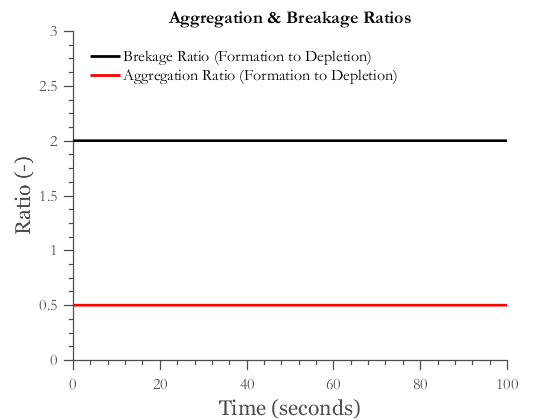
\includegraphics[scale=0.5]{rslts_anik_pbm_ratios}
\caption{Ratio of formation-to-depletion through aggregation over time for the stand alone PBM. An aggregation ratio of 0.5 indicate mass conservation in the model. \textcolor{cyan}{place holder need matlab version of fig from Chai} }
%\caption{hello tesh}
\label{fig:rslts_anik_pbm_ratios}
\end{figure}

\par To check the model for consistancy the particle formation to particle depletion ratio is collected and plotted in figure \ref{fig:rslts_anik_pbm_ratios}. In aggregation two particles agglomerate to form one particle which should give a ratio of 0.5. In breakage one particle breaks to form two particles which should give a ratio of two. However since the stand alone PBM has a breakage constant of zero the breakage ratio of particles formed to depleted was not collected. As can be seen from figure \ref{fig:rslts_anik_pbm_ratios}, the aggregation ratio of particles formed to depleted is 0.5 which confirms that mass is conserved in the stand alone PBM.

\textcolor{orange}{might take out the stuff about d50s}
\textcolor{cyan}{this is the last part I need to write up and or get the data for and or remove}
\textcolor{cyan}{also note these figs are still place holder figs for not the model that I ran in parallel so the time scales and compartment numbers are out of sync with the actually stand alone PBM I am talking about in this supplementary material section.}
\par The granulator was divided into 16 compartments spatially and the total volume, solid volume and pore volume and the median diameter $d_50$ in each compartment were plotted to study the granulation behaviour and are shown in Figure \ref{fig:rslts_anik_pbm_total_vol_solid_pore_d50}.


\par It can be seen from Figure \ref{fig:rslts_anik_pbm_total_vol} that the total volume starts to increase first in compartment 1 followed by compartment 2 and then compartment 3. This happens as gradually particles entering compartment 1 moves to the other compartment due to particle transfer from compartment 1 to compartment 2 and then compartment 3. In Figure \ref{fig:rslts_anik_pbm_total_solid_vol} it is observed that the solid volume similar to the total volume increases first in compartment 1 and last in compartment 3. The solid volume becomes constant and equal in all the compartments at around 30-50 seconds and steady state is reached when the rate of particle volume being transported through the compartments and leaving the system is equal to the rate of particles entering the system. Although, as seen in Figure \ref{fig:rslts_anik_pbm_total_pore_vol} the pore volume which is the sum of the gas and the liquid volume is highest in compartment 3 and lowest in compartment 1. This happens due to the external liquid addition to the system. As the particles move from compartment 1 to compartment 3, they gradually acquire a higher amount liquid, thereby increasing the pore volume. In Figure \ref{fig:rslts_anik_pbm_d50}, the $D_50$ is seen to be increasing from compartment 1 to 3. This happens because of the size enlargement of large particles coming in from the previous compartment because of the external liquid added to each compartment and a longer residence time in the granulator.
\textcolor{orange}{could possibly remove up to here}


\begin{figure}[H]
\centering
\begin{subfigure}[b]{0.45\textwidth}
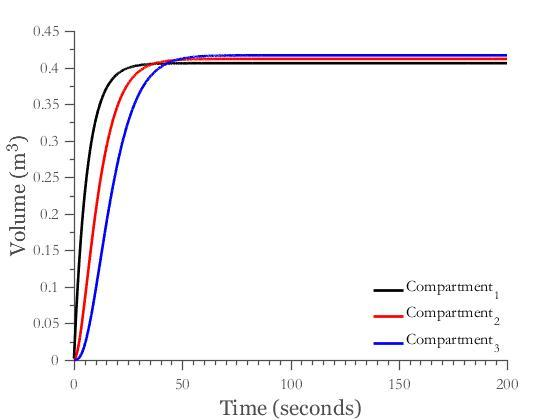
\includegraphics[width=\textwidth]{rslts_anik_pbm_total_vol}
\caption{Total volume in all compartments}
\label{fig:rslts_anik_pbm_total_vol}
\end{subfigure}
~ %add desired spacing between images, e. g. ~, \quad, \qquad, \hfill etc. 
%(or a blank line to force the subfigure onto a new line)
\begin{subfigure}[b]{0.45\textwidth}
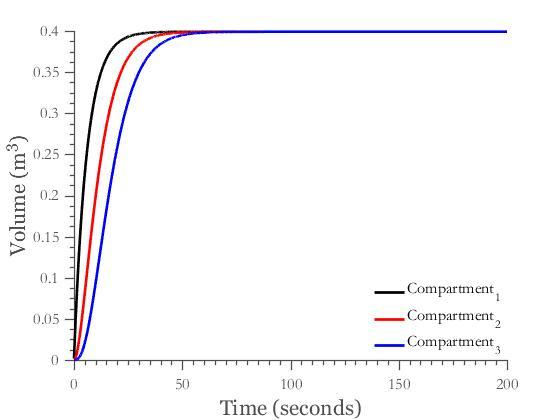
\includegraphics[width=\textwidth]{rslts_anik_pbm_total_solid_vol}
\caption{Total solid volume in all compartments}
\label{fig:rslts_anik_pbm_total_solid_vol}
\end{subfigure}
~ %add desired spacing between images, e. g. ~, \quad, \qquad, \hfill etc. 
%(or a blank line to force the subfigure onto a new line)

\begin{subfigure}[b]{0.45\textwidth}
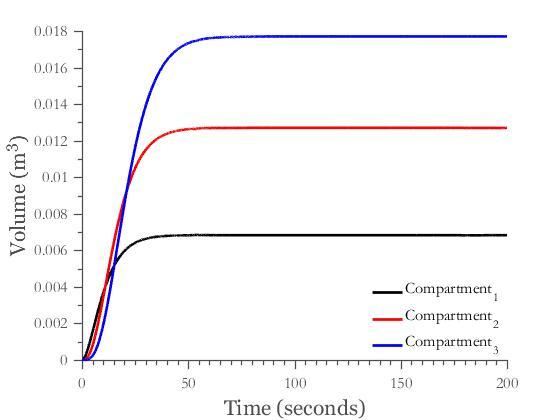
\includegraphics[width=\textwidth]{rslts_anik_pbm_total_pore_vol}
\caption{Total pore volume in all compartments}
\label{fig:rslts_anik_pbm_total_pore_vol}
\end{subfigure}
\begin{subfigure}[b]{0.45\textwidth}
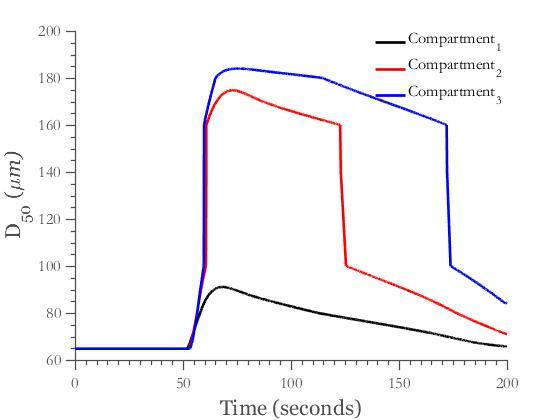
\includegraphics[width=\textwidth]{rslts_anik_pbm_d50}
\caption{D$_{50}$ in all compartments}
\label{fig:rslts_anik_pbm_d50}
\end{subfigure}

\caption{Volume and D50 in all compartments over time. Volumes become constant as steady state is reached. Median diameter increases and then decreases as bigger particles leave the system and smaller particles occupy that volume.}\label{fig:rslts_anik_pbm_total_vol_solid_pore_d50}
\end{figure}


\subsubsection{Supp. Stand Alone PBM Performance}
\label{sec:supp_sa_pbm_performance}
The stand alone PBM was run on the Stampede1 cluster located at TACC, University of Texas, Austin. The hardware configuration of each node 
consists of 2 8-core Intel Xeon E5-2680 processors based on the Sandy Bridge architecture, 32 gb of memory with QPI interconnects at 8.0 GT/s PCI-e lanes. The code was compiled using the intel v15.0.2 compiler with the -O3 option and the MPI implementation used was mvapich2/2.1. The stand alone code was run with 1 to 128 cores to test the performance. One MPI process was bound to each socket and each MPI process spawned 8 OpenMP threads ( one for each core). To account for socket affinites the "tacc affinity" option was used when running the jobs on the cluster. 


\begin{table}[H]
\caption{Performance studies of the PBM without the DEM data}
\label{table:rslts_performance_DEM_without_DEM}
\begin{center}
\begin{tabulary}{\linewidth}{C|C|C|C|C|C}
\hline
\bf{Cores in Parallel}&\bf{MPI Processes}&\bf{OMP Threads}& \bf{Wall Time (seconds)}&
\bf{SpeedUp}& \bf{Parallel efficiency}\\
\hline
$1$ & $1$ & $1$ & $222$ & $1.000$ & $1$\\
$2$ & $1$ & $2$ & $147$ & $1.510$ & $0.755$\\
$4$ & $1$ & $4$ & $109$ & $2.037$ & $0.509$\\
$8$ & $1$ & $8$ & $103$ & $2.155$ & $0.269$\\
$16$ & $2$ & $8$ & $41$ & $5.415$ & $0.338$\\
$32$ & $4$ & $8$ & $21$ & $10.571$ & $0.330$\\
$64$ & $8$ & $8$ & $10$ & $22.200$ & $0.347$\\
$128$ & $16$ & $8$ & $6$ & $37.000$ & $0.289$\\
\hline
\end{tabulary}
\end{center}
\label{table:rslts_sa_pbm_perf}
\end{table}


The parallel performance data for this model can be seen in table \ref{table:rslts_sa_pbm_perf}. The wall time was reduced from 222 seconds on one core to 6 seconds on 128 cores. The granulation process being modeled would run for a total of 90 seconds which means that the simulation ran nearly 15 times faster than the real granulation process. This is especially notable since the stand alone PBM used in this work had a significant amount of detail uisng four dimensions and two lumped parameters. 


\begin{figure}[H]
\centering
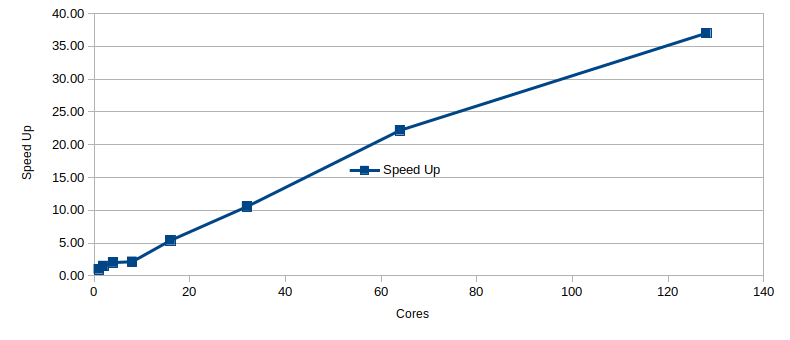
\includegraphics[scale=0.5]{fig_rslts_sa_pbm_speed_up.png}
\caption{Speed Up of stand alone PBM using 1 to 128 cores on Stampede1. \textcolor{cyan}{place holder need matlab version of fig from Chai} }
%\caption{hello tesh}
\label{fig:rslts_sa_pbm_speedup}
\end{figure}

The speed up of the stand alone PBM  is shown in figure \ref{fig:rslts_sa_pbm_speedup}. The scaling of the model was good reaching 37 times speed up when using 128 cores. The parallel efficiency drops off more quickly at lower core counts before it stabalizes at 16 cores which is a full node on Stampede1. After the first 16 cores the parallel efficiency only slightly decreases and achieves a 28.9$\%$ efficiency at 128 cores.


\begin{figure}[H]
\begin{center}
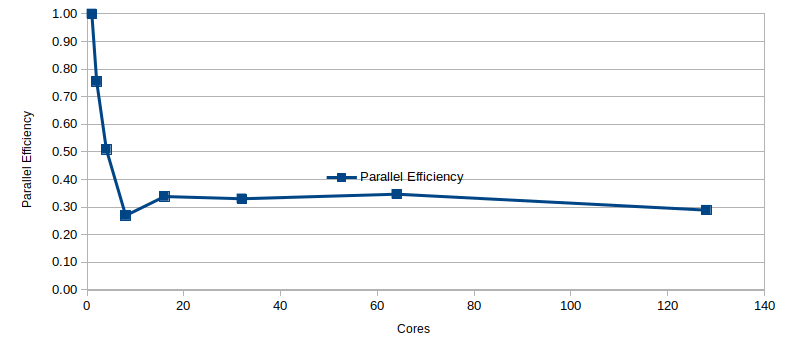
\includegraphics[scale=0.5]{fig_rslts_sa_pbm_parallel_efficiency.png}
\caption{Parallel efficiency of stand alone PBM using 1 to 128 cores on Stampede1. \textcolor{cyan}{place holder need matlab version of fig from Chai} }
\label{fig:rslts_sa_pbm_pll_effic}
\end{center}
\end{figure}

Parallel efficincy of the stand alone PBM is shown in figure \ref{fig:rslts_sa_pbm_pll_effic} for 1 to 128 cores. The model looses efficieny somewhat quickly from 1 to 8 cores as more OMP threads are introduced. From 8 to 16 cores the efficincey increases as the MPI is introduced to divide the PBM spatially. From 16 cores on out to 64 cores an efficincy of about 0.34 is maintined which suggests a good parallelization methodology. As the model is scaled from 64 to 128 cores the efficincy declines slighly as the number of MPI processes and thus message passing is doubled but still maintiains a good efficincy of 0.289.  

The scaling results for this stand alone PBM show good performance and suggest that the hybrib MPI+OMP approach worked well. It also shows that it was effective to parallelize the nested loops of the aggregation rate process calculations using OMP since they were linearized static arrays. Since the model was able to run so much faster than the real physical granulation process this stand alone PBM shows promise for optimization studies, paramter tuning studies, control strategy studies, and general QbD applications.


\subsubsection{Supp. DEM Scripts}

